
\begin{refsection}

\newrefcontext[sorting=ynt]

\lettrine{B}{irds} are unique in moving mostly by powered flight on feathered wings.
Feathers, unlike animal hair and claws, are dead proteinaceous structures, and they cannot be renewed continuously as they suffer wear and tear \cite{rayner1988,jenni1989}.
This means that as feathers mature, the wing condition and consequently flight capacity of birds is reduced \cite{lindstrom1994,hedenstrom1999,hedenstrom2003}.
Maintaining wing condition through molt --- the shedding of old, worn-out feathers, and their replacement with freshly grown ones --- is thus a key process in avian ecology \cite{ginn1983,rayner1988}.
During wing molt, as one or more old feathers are lost and new ones grow in their place, bird's flight surface becomes smaller.
The reduction in flight surface size can be measured using a robust-cross species measure index \citep{lind2001,kiat2016}, which refers to the size of the gap in the flight surface during the molt process.
Greater gap leads to temporary reductions in wing surface area, power output, and flight capacity and efficiency in captive birds \cite{tucker1991,swaddle1996,swaddle1997,williams2003,lind2001,lind2001a,bowlin2009}.
In addition to these indirect costs, wing molt can be among the most energetically demanding phases of a bird's annual cycle, as substantial resources must be channelled towards regrowing large flight feathers \cite{lindstrom1993,newton2009,kiat2017}.
% This makes the optimal movement strategy during molt unclear: whether to move more to find high-quality resources, or move less to save energy for regrowing flight feathers.
% This leaves birds in a dilemma: the increased need to move to find high-quality resources coincides with a period of reduced flight capacity and efficiency, and presumably increased vulnerability to predation.
Despite these clear mechanistic links between molt and movement, our understanding of the movement strategies and habitat selection of molting birds in the wild is poor.

Most of what we know about the influence of wing molt on the movement and habitat preferences of birds comes from a limited number of studies on migratory species.
In a few related northerly species of finches and buntings, wing molt leads to reduced movement as birds seek shelter from disturbances in vegetation or rough terrain \citep{bell1970,haukioja1971,green1975,francis1991}.
Moving less could both help avoid being detected by predators, and save energy required to regrow feathers.
Similarly, among larger waterbirds such as geese, grebes and flamingos, simultaneous molt of flight feathers renders birds flightless \citep{kiat2021}, leads them to remain near bodies of water where they can escape most predators, and results in active selection for high-quality food sources \citep{madsen1987,fox1998}.
% Consequently, the trade-offs between moving more to find high-quality resources, and moving less to save energy, and preferring resource-rich versus more sheltered habitats, are challenging to resolve.
Across these species, the molting period is usually constrained by the short time available for molt as a result of migration \citep{kiat2019} or large body size \citep{kiat2021a,jenni2020}.
% Thus even among passerines, many flight feathers are lost simultaneously, often leaving birds effectively flightless \citep{bell1970,haukioja1971,green1975,francis1991}.
This makes it difficult to separate the influence of migration and body size --- which also requires substantial resources \cite{alerstam1990,wikelski2003,horvitz2014a} --- from that of molt on habitat selection and movement decisions.
% The transition between large species (waterbirds) and northern species in this paragraph is not clear to me - I hope the edit I made matches the original intent.

A more robust comparative approach would be to quantify the effects of wing molt in a set of unrelated, non-migratory species that are not constrained by short time available for molt of northern temperate regions.
A modern, cross-species study of movement and habitat selection among molting birds can benefit from dramatic advances in the high-throughput position tracking of small species \cite{toledo2020} (Nathan et al. \textit{Science}), and from the use of standardised data pre-processing and analysis pipelines \cite{gupte2021b}.
Comparing selection for sheltered habitats across species requires using very general predictors, such as the normalised difference vegetation index (NDVI), which could indicate sheltering vegetation \cite{pettorelli2011}.
A more mechanistic approach is to actually quantify whether birds can be seen by potential predators, i.e., whether they are in the predator viewshed \cite{aben2018,aben2021}, also called a `fearscape' \cite{olsoy2015}.
Generating fine-scale viewsheds needs high-resolution ($<$ 1m) models of the landscape surface; these can pick up fine variation in vegetation height that create the small-scale habitat complexity that provides shelter.

We present a first exploration of the direct effects of wing molt on the movements of four sympatric, non-migratory, sub-tropical species: House Sparrows (\textit{Passer domesticus}), White-spectacled Bulbuls (\textit{Pycnonotus xanthopygos}), Clamorous Reed Warblers (\textit{Acrocephalus stentoreus}), and Barn Swallows (\textit{Hirundo rustica}).
We combined high-throughput tracking, experimental manipulation, and high-resolution viewshed analysis to study how molt affected birds' preferences for sheltered habitats in an agricultural-natural mosaic, in the Hula Valley, Israel.
We scored the size of the gap in the wing flight surface \citep{lind2001,kiat2016} of naturally molting and non-molting birds, and manipulated a subset of molting individuals by removing a number of flight feathers.
We tracked these birds using a high-throughput system \citep{toledo2014,weiser2016,toledo2020}, and we quantified the visibility index of bird' positions to determine their exposure to potential predators.
We examined \textit{(i)} how molt related gap's size affected bird movement, and \textit{(ii)} how gap's size influenced selection for more sheltered habitats.
Overall, we present a comprehensive, mechanistic look at how the structure of bird wings directly affects the movement and habitat selection of wild birds.
% Habitat selection or habitat preference?

\section*{Methods}

We studied bird molt and movement in the Hula Valley of northern Israel (33.10°N / 35.60°E), which includes reconstructed wetlands and reedbeds as well as agricultural areas (crops, plantations and fishponds; see Fig. X or Supplementary Fig. X).

\subsection*{Visibility analysis to quantify sheltered habitats}
The normalised difference vegetation index (NDVI) is widely used as a proxy for sheltered habitats due to its relation with vegetation growth \citep{pettorelli2011}.
However, it is small-scale habitat structure, such as the height and density of plants, that determines shelter availability, while NDVI is simply a correlate. 
Simply put, open cropland is unlikely to be very sheltered despite high NDVI values, while settlements and some natural habitats could have relatively low NDVI, yet be more sheltered due to small-scale structural complexity.
% However, small-scale habitat structure, such as the height and density of vegetation is a better indicator of the availability of shelter.
We took a mechanistic approach to quantifying shelter, and adopted a viewshed ecology approach to determine how visible an area was from surrounding locations \citep{aben2018,aben2021}.
We first obtained a 50cm digital surface model (DSM) of the majority of our study area (courtesy of the Israeli Mapping Service).
For each cell of the raster layer, we calculated a \textit{visibility index}, which is the proportion of surrounding cells from which the focal cell is visible, given that lines of sight can be blocked by intervening structures (also called cumulative viewshed analysis, or a `fearscape') \cite{olsoy2015}.
% Open areas, such as agricultural fields or water bodies are likely to be visible from all directions, and have a visibility score $\approx$ 1.0.
% In contrast, locations inside woodland or reedbeds are likely to be hidden from view, with a lower visibility index (see Supplementary Material Fig. X).
Importantly, the visibility index depends on the height above surface level of the hypothetical observer; observers higher up may be able to see locations that are obstructed from a terrestrial viewpoint.
We calculated our visibility index based on the hunting flight of a common raptor, the low-flying Eurasian sparrowhawk (\textit{Accipiter nisus}), and assumed an observer height of 1.5m above surfaces (tree canopy or fields), and an observer visual range of 50m.

\subsection*{Bird capture and wing molt scoring}

We captured N individuals of four species in 2016: N common sparrows (\textit{Passer domesticus}), N white-browed bulbuls (\textit{Pycnonotus xanthopygos}), N clamorous reed warblers (\textit{Acrocephalus stentorious}), and N barn swallows (\textit{Hirundo rustica}).
We captured all individuals before the molting season commenced but after breeding was completed, between June and mid-November 2016.
% and ending immediately after molt completed. 
We first described the state of each primary feather on a scale of 0 to 5 using the primary score (PS) method \citep{ginn1983}.
On this scale, both PS = 0 and PS = 5 indicate a fully mature feather, and hence no gap in the wing, while a PS between 1 and 4 indicate feathers in increasing stages of maturation, with PS = 1 representing a large gap left by a recently molted feather.
% Here PS = 0 is a mature feather ready to molt, PS = 1 is a gap caused by a recently molted mature feather, or by a new feather that is found completely within its pin. 
% PS = 2 is a new feather just emerging from its sheath, up to the length of a one third of a fully grown feather. 
% PS = 3 is a new feather with a length between one and two thirds of a fully grown feather, while PS = 4 is a new feather that is more than two thirds the length of a fully grown feather and with remains of waxy sheath at its base.
% Finally, and PS = 5 is a new, fully developed feather with no traces of remaining waxy sheath at its base.
% To estimate the molt speed of each individual
To compare molt molt related wing's gap size across individuals, we sum the values for all primary flight feathers \citep{kiat2016}. 
This method estimates the size of the feather gap in the wing caused by molt and also strongly and negatively correlated with molt speed and duration \citep{rohwer2009}. 
This score is the inverse value of PS for each of the wing's nine primary feathers (P1-P9; counted outward) such that when PS = 1, gap size = 4, and when PS = 2, gap size = 3, etc. 
However, for PS = 0, gap size is also 0 because there is no gap in both the PS = 0 and PS = 5 stages, as either an old, mature feather, or a new, freshly grown feather is present.
We calculated the individual score by summing the gap sizes across all nine primary feathers. 
This score estimate is independent of bird size and morphology, controls for the stage of wing feather molt and allows for reliable cross-species comparisons \citep{bensch1993}.
Bird capture, handling, and tagging (see below) were conducted under a permit from the Israel Nature and Parks Authority (NPA permit 2016/41402) and from the ethics committee of the Hebrew University of Jerusalem (NS-16-14801-2).

\subsection*{Tracking bird movement using ATLAS}

We tracked the movement of individual birds using ATLAS (Advanced Tracking and Localization of Animals in real-life Systems), a state-of-the-art high-throughput radio-telemetry system capable of tracking dozens of individuals at intervals of 4 seconds \citep{weiser2016,toledo2014,toledo2020}.
ATLAS tags ({\color{red}X g}) were fitted to birds during the capture procedure, and birds were released after tags were attached.
Each individual was tracked for an average of X days (SD = Y days; by species, warbler: X $\pm$ Y days; sparrow: X $\pm$ Y days; bulbul: X $\pm$ Y days; swallow: X $\pm$ Y days).
We collected Nmax position estimates overall, with N positions per individual per day, for an effective tracking interval of N positions / hour on average (SD = Y positions; by species, warbler: X $\pm$ Y positions; sparrow: X $\pm$ Y positions; bulbul: X $\pm$ Y positions; swallow: X $\pm$ Y positions).
Since we were interested in exploring movement patterns, and these species are diurnally active, we removed all nighttime positions, leading to an approximate halving (as expected; \% data remaining = X\%) of the total dataset.

\subsection*{Pre-processing tracking data}

ATLAS systems can achieve a spatial resolution comparable to that of GPS position loggers \citep{beardsworth2021}, and this resolution can be improved with minimal pre-processing, or data cleaning \citep{beardsworth2021, gupte2021b}.
We began data cleaning by removing locations near a so-called attractor position (at (257000.0,780000.0), Israeli grid; see file \textit{log\_preprocessing.log}); these are locations for which the positioning system had defaulted to a (wrong) estimate.
We identified and removed other attractor positions by removing positions sharing the exact same common coordinate pair. 
Since coordinates are resolved down to double-precision, it is very unlikely for two location estimates to have the same coordinate pair, and this rather indicates an error in location estimation.
%
We then \textit{(i)} filtered the data for large-scale errors by removing positions with a system-generated positioning-error estimate (SD) $>$ 20m, and \textit{(ii)} split each individual's tracking data by calendar date, removing dates with $<$ 500 positions. We then \textit{(iii)} filtered the data for unrealistic movements using a combined filter on incoming and outgoing speed and turning angle (speed threshold = 20 m/s, angle threshold = 10 degrees).
We deliberately used larger thresholds than these species' maximum speeds to avoid removing valid, high-speed movements \citep{gupte2021b}.
Finally, we \textit{(iv)} accounted for small-scale errors --- noise around the true positions --- by applying a median smooth with a moving window $K$ = 7.
Each individual's track was pre-processed separately and completely cleared before the next individual was handled, to reduce mix-ups.

\subsection*{Quantifying large-scale movements}

We investigated the large-scale space-use of reed-warblers, sparrows, and bulbuls by summarising their pre-processed movement paths into daily sequences of `residence patches' using the \textit{atlastools} package developed specifically with high-throughput ATLAS tracking data in mind \citep{gupte2021b}.
The residence patch algorithm uses simple distance and duration thresholds, chosen based on the movement ecology of the tracked species, to efficiently and rapidly cluster-segment individuals' non-travelling positions \citep{gupte2021b}.
We applied this algorithm to the date-specific tracks of each individual, considering consecutive positions less than 25m and 30 minutes apart to be part of the same cluster, and joining clusters (with at least 9 positions) less than 100m and 30 minutes apart together.
Doing so, we obtained 4,xxx residence patches overall.
We constructed 25m buffers around the positions in each cluster, and used the buffers to obtain summary statistics of the environmental layers (NDVI, landcover, and visibility) for each patch.
%%
We handled swallows differently, as these are highly aerial birds whose movement is not easily clustered into residence patches.
Instead, and because the relatively higher-flying swallows are more accurately tracked by ATLAS, we simply calculated the total distances moved along daily tracks from the cleaned, pre-processed data.
% Instead, we fitted continuous-time movement models to the daily movement tracks of each swallow, using the \textit{ctmm} package; the \textit{ctmm} package's model selection procedure automatically selects the best model from among multiple options based on AICc differences \citep{fleming2014,fleming2015,calabrese2016}.
% We used these fitted models to calculate the daily distance moved by each swallow.
% We obtained daily 95\% autocorrelated kernel density estimates (AKDE) of the utilisation distributions of each swallow, using the weighted AKDE method suitable for relatively sparsely sampled tracks \citep{silva2021}.

\subsection*{Drawing alternative residence patches to examine habitat selection}

% Large-scale analyses showed a strong negative correlation between NDVI and visibility within residence patches (see Supplementary Material Fig. X).
To disentangle the effects of shelter and vegetation growth on individual's movement decisions, we combined our residence patch approach with step-selection analysis \citep{thurfjell2014,avgar2016} using the \textit{amt} package \citep{signer2019}.
We converted each individual's daily sequence of residence patches into steps, with patch $i$ as the starting point, and patch $i+1$ as the end.
For each such real step, we drew 9 alternative steps that the individual could have taken from patch $i$, and we considered the end coordinates of these alternative steps to represent the median coordinates of a potential residence patch (see Supplementary Material Fig. X).
The distances of these movements were drawn from a gamma distribution fitted to each individual's movements between patches, and turning angles were drawn from a von Mises distributions fitted to the observed turning angles \citep{signer2019}.
%%
We sampled the NDVI and visibility of each real patch at the tracked positions which had been clustered into that patch \citep{gupte2021b}.
For each alternative patch with median coordinates ($X_{alt}, Y_{alt}$), we drew 5 coordinate pairs from a normal distribution centred on ($X_{alt}, Y_{alt}$), and sampled the NDVI and visibility at each location.
%%
Essentially, we were able to compare a flexible number of $N$ positions that were clustered into a residence patch $i$, against 9 $ \times$ 5 = 45 coordinates of \textit{patches that could have been}, i.e., clusters of locations the bird could have occupied.
% NDVI cannot be used to distinguish ares of natural vegetation from agriculture in our mixed land-use study site.
% To control for qualitative differences in vegetation, we also obtained the proportion of natural or artificial land-cover types at the start and end of each step (natural: X, artificial: Y).
% We then fit integrated step selection functions to daily individual tracks, with the model formula \textit{case $\sim$ log\_sl + visibility + ndvi + ndvi:visibility + strata(step\_id)}.
% Here \textit{case} is a binary outcome indicating an actual (True) or potential step (False), \textit{log\_sl} is the log step length, and \textit{strata(step\_id)} controls for step-specific variation.

\section*{Results}

\subsection*{Molt related gap's size determines movement in wide ranging species}

Of the four species we studies, bulbuls and sparrows are relatively wide-ranging terrestrial birds, reed-warblers are strongly range restricted to patchy reedbeds, and swallows are very wide-ranging, largely aerial birds.
Bulbuls and sparrows adjusted their large scale movements between areas of prolonged residence (`residence patches', see Fig.~\ref{fig1}) \cite{gupte2021b}, to their wing gap's size.
Naturally molting bulbuls and sparrows with moderately molt related gap's size (3 $<$ wing gap $\leq$ 10) actually moved more per hour between residence patches (estimate = 19.64, p = 0.007), than non-molting individuals (wing gap = 0).
This is consistent with the idea that wing molt is an energetically demanding period that requires actively seeking out high-quality food sources \citep{madsen1987,fox1998}.
However, bulbuls and sparrows whose flight feathers had been removed by manipulation (15 $<$ wing gap $<$ 20) moved less than naturally molting birds; bulbuls especially did not move at all when their wings were heavily compromised (wing gap $>$ 15).
This is in line both with a direct effect of severely reduced flight capacity, and an indirect effect of risk-avoidance during a vulnerable period.
Similarly, naturally molting swallows moved more than non-molting swallows, and swallows with wing feathers removed moved less than either non-molting or naturally molting individuals (Fig.~\ref{fig2}).
Reed-warblers, on the other hand, did not appear to move more when molting naturally, but like bulbuls, moved very little between patches when their wing's gap were larger (wing gap $>$ 15; Fig.~\ref{fig1}).
This may be because reed-warblers are already very strongly constrained to a few clustered reedbed habitats, and thus do not move between distant patches even when not molting.
Overall, this suggests that these species' movement strategies switch between resource-maximising (when molting naturally) and risk-minimising (when manipulated), depending on how compromised the wing surface is.

\begin{figure}[!h]
    \centering
    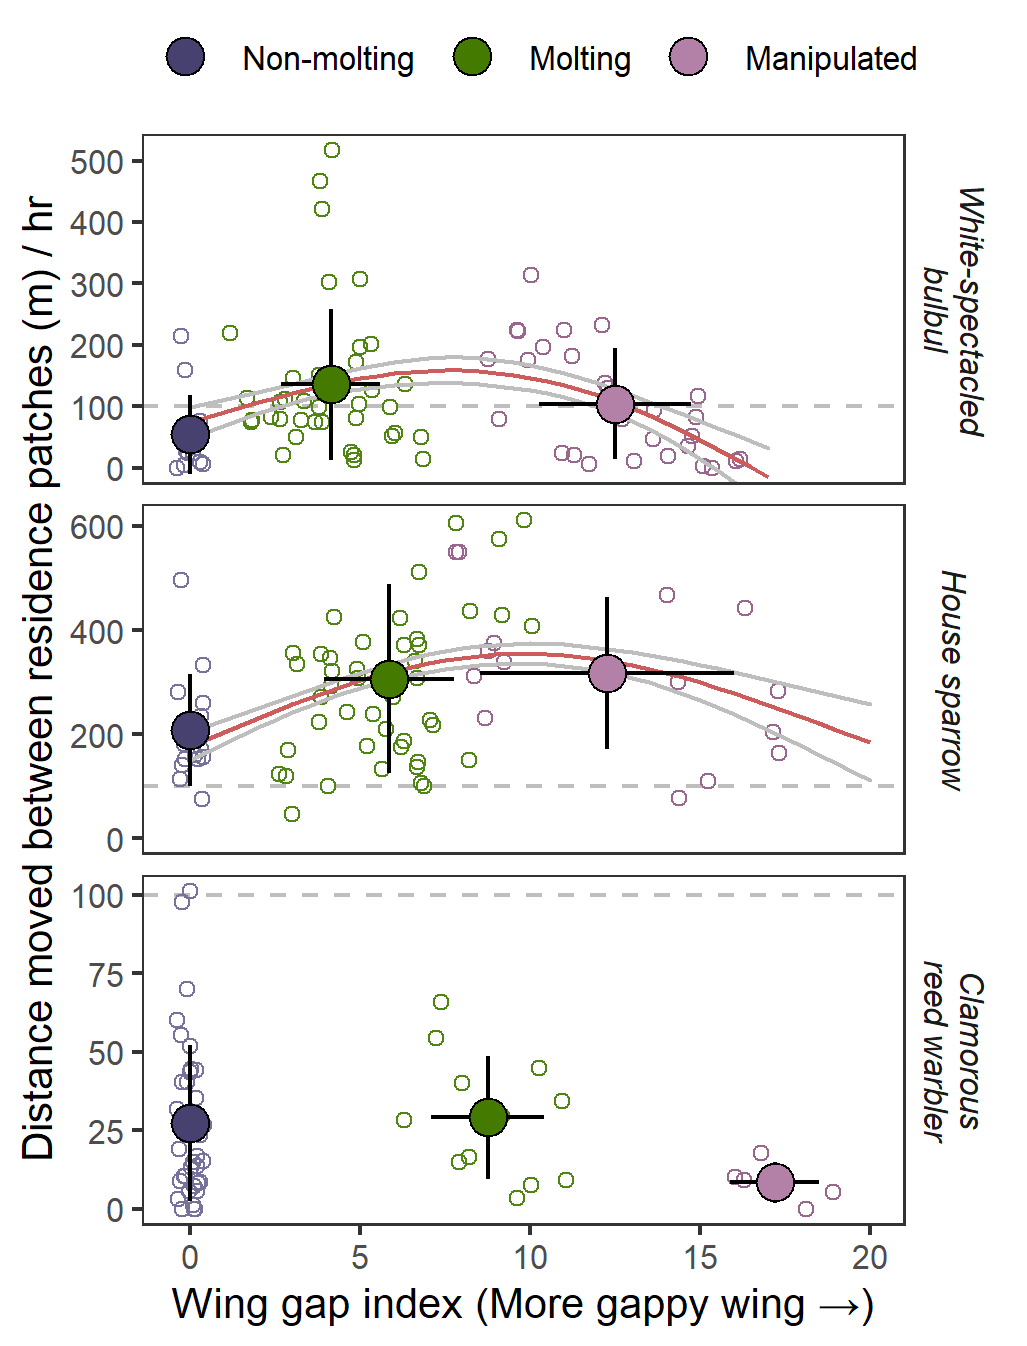
\includegraphics[width=0.9\textwidth]{figures/holeybirds/fig_01.png}
    \caption{
        \textbf{Increased movement during natural molt, but reduced movement following manipulation in reed-warblers, sparrows and bulbuls.}
    }\label{moult_fig_01}
\end{figure}

\begin{figure}[!h]
    \centering
    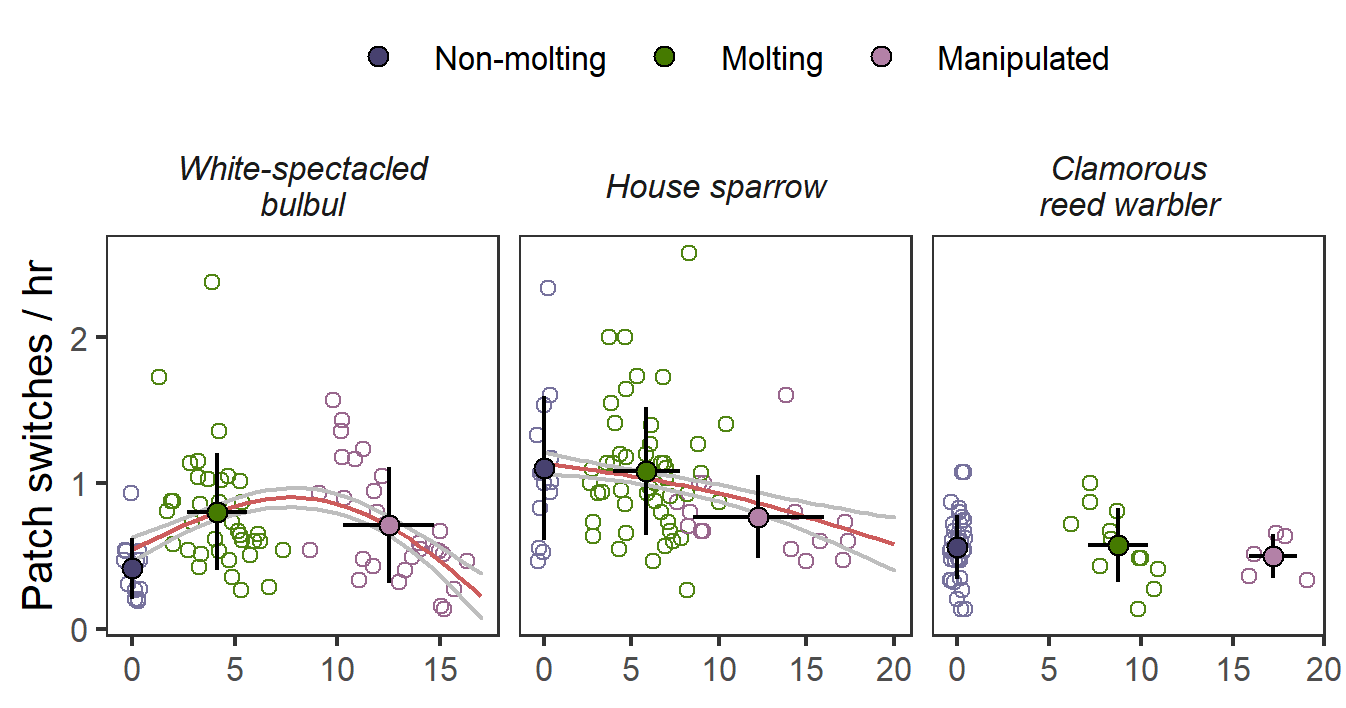
\includegraphics[width=0.9\textwidth]{figures/holeybirds/fig_02.png}
    \caption{
        \textbf{Increased movement during natural molt, but reduced movement following manipulation in swallows.}
    }\label{moult_fig_02}
    \end{figure}

\subsection*{Birds select for sheltered viewsheds, regardless of molt status or vegetation}

Individuals of all three terrestrial species mostly had most of their residence patches in relatively low-visibility areas (visibility $\leq$ 0.5; Fig.~\ref{fig3}).
This indicates locations which can, at most, be observed from only half of surrounding locations by a predator up to 50m away and at a height of 1.5 metres above the surface --- such as a low-flying predatory bird (e.g. Eurasian sparrowhawk \textit{Accipiter nisus}).
This is consistent with most individuals' use of patches of natural vegetation (such as reedbeds) or semi-natural agriculture (such as orchards) in our landscape.
Birds' use of sheltered areas was only moderately related with the size of molt related wing's gap.
Naturally molting reed-warblers used more sheltered areas than non-molting ones, and manipulated individuals used more sheltered areas than even naturally molting ones (Fig.~\ref{fig3}).
Bulbuls were similar to reed-warblers in being restricted to habitats with trees, with a low average visibility $\approx$ 0.25.
In contrast, manipulated sparrows with larger wing gap used more open areas than either non-molting or naturally molting individuals (Fig.~\ref{fig3}).
Sparrows are more widespread in our landscape than reed-warblers, and being smaller than bulbuls may be less easily spotted by predators when they venture into more open areas.
We found that regardless of molt related gap size, and when considering relatively well-vegetated habitats (NDVI $>$ 0.4), all three of these terrestrial species preferred low-visibility sites over higher visibility ones (Fig.~\ref{fig3}).

\begin{figure}[!h]%[\sidecaptionrelwidth]
    \centering
    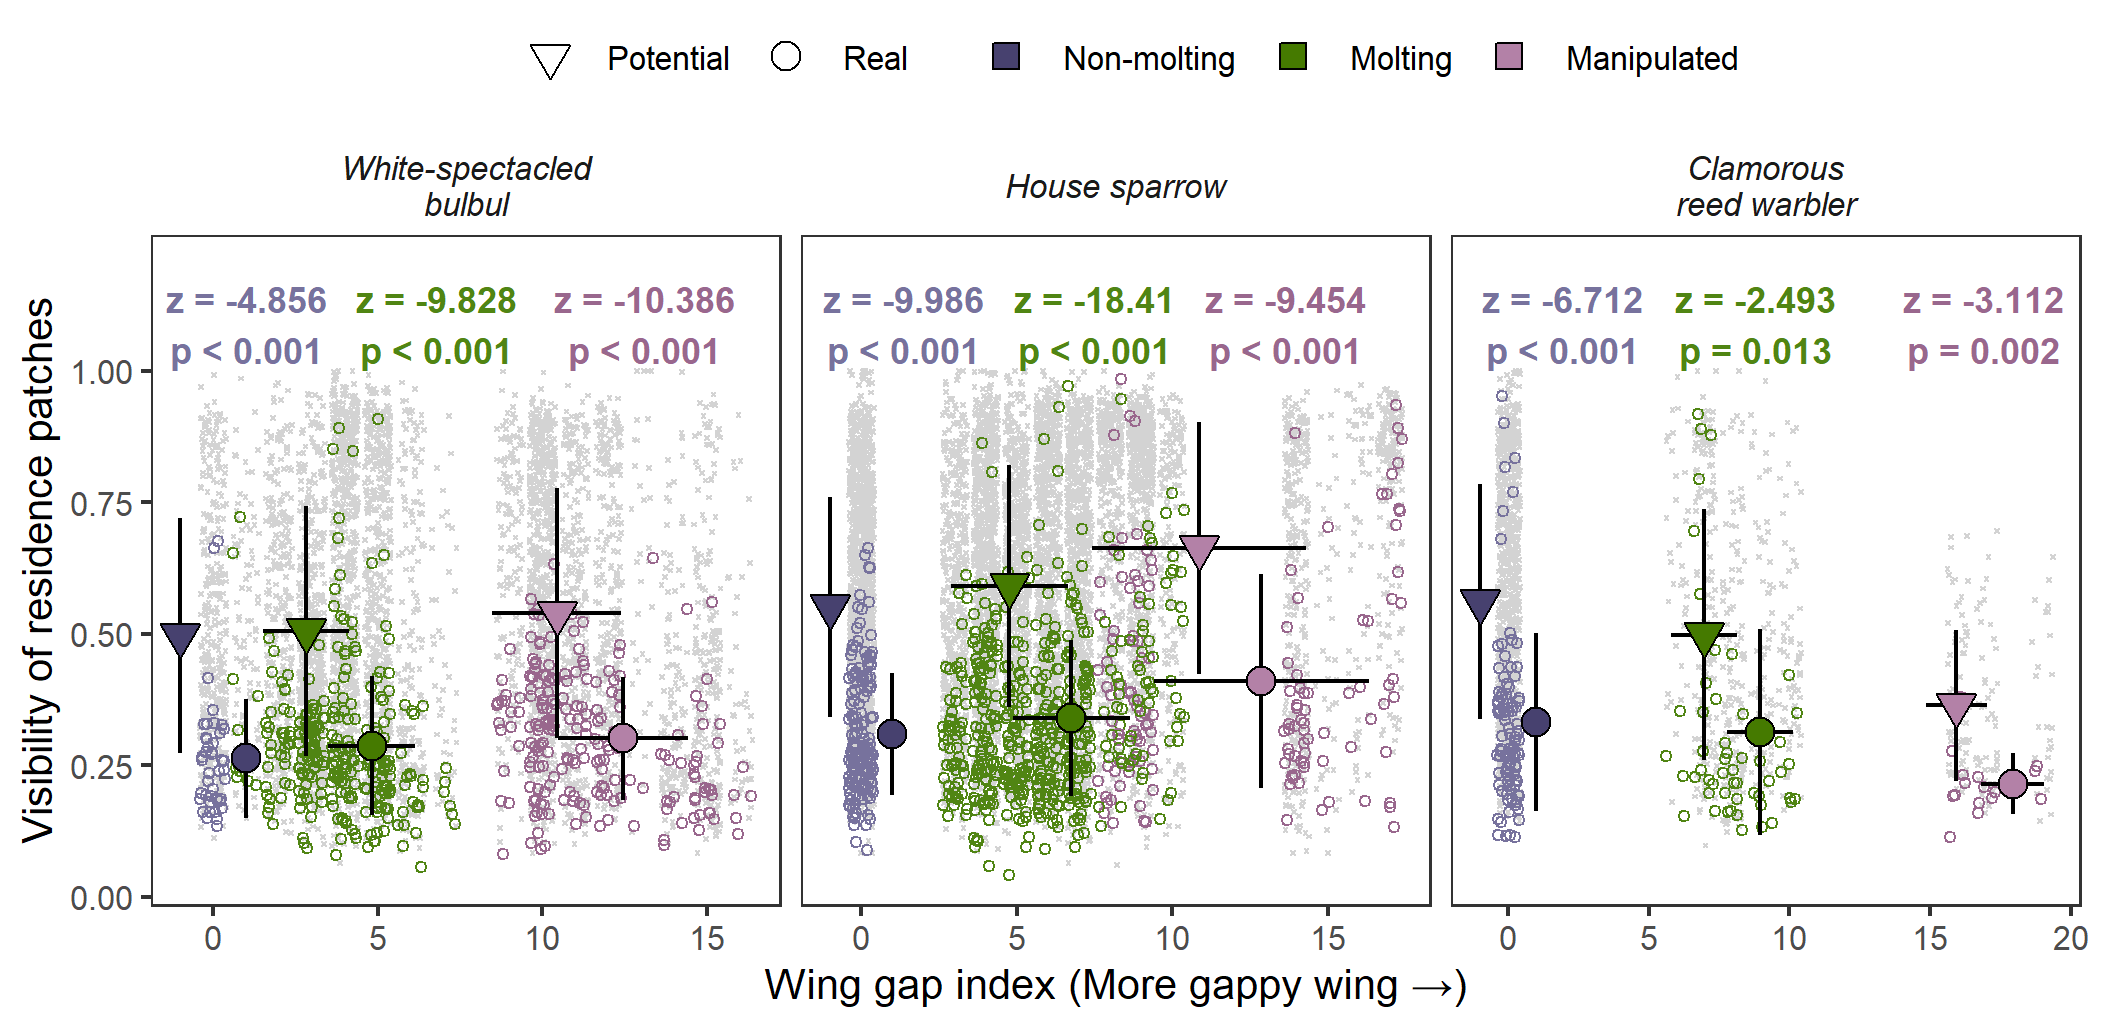
\includegraphics[width=0.9\textwidth]{figures/holeybirds/fig_03.png}
    \caption{
        \textbf{Reed-warblers, sparrows and bulbuls prefer sheltered habitat even within high-productivity areas.}
    }\label{moult_fig_03}
\end{figure*}

% \subsection*{Land-use determines whether increased vegetation leads to sheltered viewsheds}

% Our study site is comprised of a mixture of land-use types, and many of these are associated with vegetation (reedbeds and orchards), or rapid vegetation growth (agricultural fields).
% However, shelter from the view of predators is a function of habitat micro-structure, and in vegetated habitats, of the morphology of plants.
% Agricultural fields especially have large NDVI values (mean = X, sd = X), reflecting the rapid vegetation growth associated with crop plants; however, most crops plants are not particularly tall (mean surface height = X, sd = X), and these is little heterogeneity in plant height within fields.
% Consequently, these open fields have very high visibility (mean vis = X, sd = X), and likely provide little shelter, especially from aerial predators.
% In contrast, areas under natural vegetation or with orchards have substantially taller plants (mean = X, sd = X); these natural habitats are thus much more sheltered, even from aerial observation (mean vis = X, sd = X).
% Surprisingly, completely anthropogenic features, such as houses in settlements, can also create quite sheltered areas (mean vis = X, sd = X), as the height and placement of houses obstructs lines of sight.
% Overall then, we find that in agricultural mosaics, the interaction of landcover and NDVI determines the viewshed of a location, and whether that location provides any shelter to wildlife.

% \begin{figure*}%[\sidecaptionrelwidth]
% \centering
% \includegraphics[width=17.8cm,height=8.7cm]{figures/fig_01_02.png}
% % width=8.7cm,height=8.7cm
% \caption{
%     \textbf{Land cover determines the coupling of vegetation growth and the availability of sheltered viewsheds in an agricultural mosaic.}
%     In our study site, \textbf{(A)} the normalised difference vegetation index (NDVI) correlates with \textbf{(B)} sheltered viewsheds only in \textbf{(C)} natural habitats, but not in agricultural areas.
%     The relatively low plant height in crop fields results in open landscapes with little cover from predators, while natural areas have more variation in plant height, which contributes to lower visibility, and potentially more shelter.
%     Settlements are also relatively sheltered, as houses obstruct lines of sight.
% }\label{fig1}
% \end{figure*}

\section*{Discussion}

Our study is among the first to quantify how the compromised wing surface associated with molt affects movement and habitat selection among wild birds, and indeed to study the effects of molt in sub-tropical species.
It was not surprising to find that three of our four species --- bulbuls, sparrows, and swallows --- moved more when their wing's flight surface is reduced and flight feathers are growing during the molt process, but that these species moved substantially less when their wings were severely compromised due to artificial manipulation.
Birds can compensate for lower wing power output by growing their pectoral muscles, allowing them to maintain flight capacity during molt, and enabling increased movement to find resources for feather growth \cite{chai1997,swaddle1997}.
When birds cannot compensate the costs of inefficient flight and feather growth through increased movement for resources --- such as when artificially manipulated --- moving less overall may be the optimal strategy until new flight feathers develop.
This may also explain why clamorous reed warblers, which molt several flight feathers in short time intervals, make shorter movements with increasing wing gap \cite{kiat2016}.

We have also for the first time applied the idea of the cumulative viewshed to directly assess the availability of shelter along birds' real and potential movement paths \cite{olsoy2015}.
All three terrestrial species strongly preferred sheltered, low-visibility habitats over more open sites, even when the available sites had similar vegetation productivity.
One the one hand, this may be because areas which are both open and have high plant productivity --- primarily agricultural fields --- are simply unsuitable for our species.
For instance, intensive monocultures may not support as many prey species, or may come with frequent disturbances.
On the other hand, our work suggests that avoidance of high-visibility areas may be an overlooked mechanism by which agricultural `green deserts' exclude avian biodiversity, though the idea is applicable across taxa.
A learned or evolved unwillingness to break cover from sheltered areas, and move through high-visibility habitat, may explain how individual movement decisions can scale up to restrict animal space-use, from home-ranges to dispersal kernels.

Birds' avoidance of high-visibility areas raises the intriguing possibility that avian spatial cognition extends to `spatial perspective taking'.
This means birds may be able to compute whether a location is visible from the perspective of another observer, such as a predator \cite{olsoy2015}.
Previous work on animal viewsheds has focussed on movement and habitat selection in relation to individual lines of sight \cite{krams2001,aben2021}.
Our study shows how animal movement decisions can also incorporate individuals' estimates of what \textit{other animals} can see \cite{kopp1998}.
The use of 
Modelling individual-specific and individual-exclusive viewsheds may also help explain the mechanistic underpinnings of fine-scale behaviours, such as intra-specific competition.
At a larger scale, visibility analysis provides a simple, mechanistic way to incorporate animals' potential assessments of landscape risk into habitat selection models.

% \subsection*{Manuscript Length}

% A standard 6-page article is approximately 4,000 words, 50 references, and 4 medium-size graphical elements (i.e., figures and tables). The preferred length of articles remains at 6 pages, but PNAS will allow articles up to a maximum of 12 pages.


% \subsection*{Supporting Information Appendix (SI)}

% Authors should submit SI as a single separate SI Appendix PDF file, combining all text, figures, tables, movie legends, and SI references. SI will be published as provided by the authors; it will not be edited or composed. Additional details can be found in the \href{https://www.pnas.org/authors/submitting-your-manuscript#manuscript-formatting-guidelines}{PNAS Author Center}. The PNAS Overleaf SI template can be found \href{https://www.overleaf.com/latex/templates/pnas-template-for-supplementary-information/wqfsfqwyjtsd}{here}. Refer to the SI Appendix in the manuscript at an appropriate point in the text. Number supporting figures and tables starting with S1, S2, etc.

% Authors who place detailed materials and methods in an SI Appendix must provide sufficient detail in the main text methods to enable a reader to follow the logic of the procedures and results and also must reference the SI methods. If a paper is fundamentally a study of a new method or technique, then the methods must be described completely in the main text.

% \subsubsection*{SI Datasets} 

% Supply .xlsx, .csv, .txt, .rtf, or .pdf files. This file type will be published in raw format and will not be edited or composed.

\newrefcontext[sorting=nyt]
\section*{Literature Cited}
\printbibliography[title={Literature~Cited},heading=none]
\end{refsection}